\documentclass{beamer}
\usepackage[utf8]{inputenc}
\usepackage[UKenglish]{babel}
\usepackage[UKenglish]{isodate}
\usepackage{tikz}
\usepackage{minibox}
\usepackage{listings}
\usepackage{complexity}

\beamertemplatenavigationsymbolsempty
\usetheme{Madrid}
\usecolortheme{orchid}

\usetikzlibrary{arrows}
\usetikzlibrary{arrows.meta}
\usetikzlibrary{positioning}
\usetikzlibrary{shapes}

\author[P. Dilkas, V. Belle]{\textbf{Paulius Dilkas} \and Vaishak Belle}
\title[WMC with Conditional Weights for BNs]{Weighted Model Counting with
  Conditional Weights for Bayesian Networks}
\date{UAI 2021}
\institute[University of Edinburgh]{University of Edinburgh, Edinburgh, UK}

\begin{document}

\begin{frame}[noframenumbering,plain]
  \tikz[remember picture,overlay]{
    \node at ([yshift=25pt,xshift=30pt]current page.south)
    {\includegraphics[height=40pt]{../poster/logo_inf.png}};
    \node at ([yshift=25pt,xshift=75pt]current page.south)
    {\includegraphics[height=40pt]{../poster/logo_ecr.png}};
    \node at ([yshift=20pt,xshift=140pt]current page.south)
    {\includegraphics[height=20pt]{../poster/logo_ukri.png}};
  }
  \titlepage
\end{frame}

\begin{frame}[fragile]{The Problem of Computing Probability}
  \vspace{-0.75cm}
  \begin{columns}[t]
    \begin{column}{0.6\textwidth}
      \centering
      \begin{block}{ProbLog}
        \vspace{-0.3cm}
        \begin{lstlisting}[basicstyle=\tiny]
0.001 :: burglary.
0.002 :: earthquake.
0.95 :: alarm :- burglary, earthquake.
0.94 :: alarm :- burglary, \+ earthquake.
0.29 :: alarm :- \+ burglary, earthquake.
0.001 :: alarm :- \+ burglary, \+ earthquake.
0.9 :: johnCalls :- alarm.
0.05 :: johnCalls :- \+ alarm.
0.7 :: maryCalls :- alarm.
0.01 :: maryCalls :- \+ alarm.
        \end{lstlisting}
        \vspace{-0.2cm}
      \end{block}
      \vspace{-0.25cm}
      \begin{block}{BLOG}
        \vspace{-0.3cm}
        \begin{lstlisting}[escapeinside={(*}{*)},basicstyle=\tiny]
random Boolean Burglary (*$\sim$*) BooleanDistrib(0.001);
random Boolean Earthquake (*$\sim$*) BooleanDistrib(0.002);
random Boolean Alarm (*$\sim$*)
  if Burglary then
    if Earthquake then BooleanDistrib(0.95)
    else BooleanDistrib(0.94)
  else
    if Earthquake then BooleanDistrib(0.29)
    else BooleanDistrib(0.001);
random Boolean JohnCalls (*$\sim$*)
  if Alarm then BooleanDistrib(0.9)
  else BooleanDistrib(0.05);
random Boolean MaryCalls (*$\sim$*)
  if Alarm then BooleanDistrib(0.7)
  else BooleanDistrib(0.01);
        \end{lstlisting}
        \vspace{-0.2cm}
      \end{block}
    \end{column}
    \begin{column}{0.35\textwidth}
      \begin{block}{Bayesian Network}
        \centering
        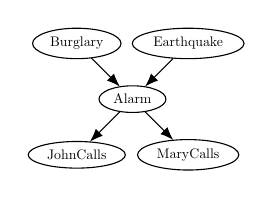
\begin{tikzpicture}[node distance=2cm,scale=0.5,every node/.style={scale=0.5}]
          \node[draw,ellipse] (alarm) {Alarm};
          \node[draw,ellipse,above left of=alarm] (burglary) {Burglary};
          \node[draw,ellipse,above right of=alarm] (earthquake) {Earthquake};
          \node[draw,ellipse,below left of=alarm] (johnCalls) {JohnCalls};
          \node[draw,ellipse,below right of=alarm] (maryCalls) {MaryCalls};
          \draw[-Latex] (burglary) -- (alarm);
          \draw[-Latex] (earthquake) -- (alarm);
          \draw[-Latex] (alarm) -- (johnCalls);
          \draw[-Latex] (alarm) -- (maryCalls);
        \end{tikzpicture}
      \end{block}
      \vspace{1cm}
      \begin{block}{Markov Random Field}
        \centering
        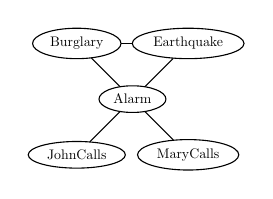
\begin{tikzpicture}[node distance=2cm,scale=0.5,every node/.style={scale=0.5}]
          \node[draw,ellipse] (alarm) {Alarm};
          \node[draw,ellipse,above left of=alarm] (burglary) {Burglary};
          \node[draw,ellipse,above right of=alarm] (earthquake) {Earthquake};
          \node[draw,ellipse,below left of=alarm] (johnCalls) {JohnCalls};
          \node[draw,ellipse,below right of=alarm] (maryCalls) {MaryCalls};
          \draw (burglary) -- (earthquake);
          \draw (burglary) -- (alarm);
          \draw (earthquake) -- (alarm);
          \draw (alarm) -- (johnCalls);
          \draw (alarm) -- (maryCalls);
        \end{tikzpicture}
      \end{block}
    \end{column}
  \end{columns}
  \onslide<2>{
    \begin{tikzpicture}[remember picture,overlay]
      \node[draw,star,fill=red!10] (wmc) at (current page.center) {WMC};
      \coordinate[xshift=-0.25\linewidth,yshift=-0.25\textheight] (p1) at (current page.center);
      \coordinate[xshift=0.25\linewidth,yshift=-0.25\textheight] (p2) at (current page.center);
      \coordinate[xshift=-0.25\linewidth,yshift=0.25\textheight] (p3) at (current page.center);
      \coordinate[xshift=0.25\linewidth,yshift=0.25\textheight] (p4) at (current page.center);
      \draw[-latex,line width=2pt,color=red!50] (p1) -- (wmc);
      \draw[-latex,line width=2pt,color=red!50] (p2) -- (wmc);
      \draw[-latex,line width=2pt,color=red!50] (p3) -- (wmc);
      \draw[-latex,line width=2pt,color=red!50] (p4) -- (wmc);
    \end{tikzpicture}
  }
\end{frame}

\begin{frame}[fragile]{Weighted Model Counting (WMC)}
  \begin{columns}
    \begin{column}{0.5\textwidth}
      \begin{itemize}
      \item Generalises propositional model counting ($\#\SAT{}$)
      \item Applications:
        \begin{itemize}
        \item graphical models
        \item probabilistic programming
        \item neural-symbolic artificial intelligence
        \end{itemize}
      \item Main types of algorithms:
        \begin{itemize}
        \item using knowledge compilation
        \item using a \SAT{} solver
        \item manipulating pseudo-Boolean functions
        \end{itemize}
      \end{itemize}
    \end{column}
    \begin{column}{0.5\textwidth}
      \begin{example}
      $w(x) = 0.3$, $w(\neg x) = 0.7$, $w(y) = 0.2$, $w(\neg y) = 0.8$
      \vspace{1cm}

      $\mathsf{WMC}(\alert{x \lor y}) = w(x)w(y) + w(x)w(\neg y) + w(\neg x)w(y)
      = 0.44$
      \end{example}
    \end{column}
  \end{columns}
\end{frame}

% BAs, pseudo-Boolean functions, measures, equivalence of definitions
\begin{frame}{An Alternative Way to Think About It}
\end{frame}

% The theorems: WMC is not expressive enough to cover all measures but can be
% extended to do so
\begin{frame}{Some Theoretical Results}
\end{frame}

% Things I could mention:
% The details of the transformation
% Experimental results

\begin{frame}{The Big Picture}
  \begin{columns}
    \begin{column}{0.35\textwidth}
      \centering
      \structure{Probabilistic Inference} \\
      (e.g., a Bayesian network)
      \fbox{
        \begin{minipage}{2.5cm}
          \centering
          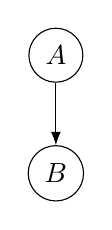
\begin{tikzpicture}[edge from parent/.style={draw,-{Latex}}]
            \node[draw,circle] at (0, 0) (a) {$A$}
            child {node[draw,circle] (b) {$B$}};
          \end{tikzpicture}\\
          Find \alert{$\Pr(B = 0)$}
        \end{minipage}
      }
    \end{column}
    \begin{column}{0.35\textwidth}
      \centering
      \structure{WMC Encoding} \\
      (CNF with literal weights)
      \framebox{
        \scalebox{0.2}{
          \begin{tabular}{@{}l@{}}
            p cnf 8 17 \\
            -2 -1 0 \\
            1 2 0 \\
            -3 1 0 \\
            -1 3 0 \\
            -5 -1 0 \\
            -5 -4 0 \\
            1 4 5 0 \\
            -6 -1 0 \\
            -6 4 0 \\
            -4 1 6 0 \\
            -7 1 0 \\
            -7 -4 0 \\
            -1 4 7 0 \\
            -8 1 0 \\
            -8 4 0 \\
            -4 -1 8 0 \\
            -4 0 \\
            c weights 1.0 1.0 0.5 1.0 0.5 1.0 1.0 1.0 0.6 1.0 0.4 1.0 0.1 1.0 0.9 1.0
          \end{tabular}%
        }
      }

      \vspace{1cm}
      \onslide<2>{
      \structure{Conditional Weights} \\
      \framebox{
        \scalebox{0.2}{%
          \begin{tabular}{@{}l@{}}
            p cnf 2 1 \\
            2 0 \\
            w 1 0.5 0.5 \\
            w 2 1 0.6 0.4 \\
            w 2 -1 0.1 0.9
          \end{tabular}%
        }
      }
      }
    \end{column}
    \begin{column}{0.30\textwidth}
      \centering
      \structure{WMC Algorithm}\\
      \onslide<2>{\alert{$>100\times$} faster}
    \end{column}
  \end{columns}
  \begin{tikzpicture}[remember picture,overlay]
    \draw[-{Latex}] (3.4, 3) -- (4.9, 4);
    \draw<2>[-{Latex}] (3.4, 3) to [bend right] (5.8, 0.2);
    \draw[-{Latex}] (7.7, 4) -- (9, 2.8);
    \draw<2>[-{Latex}] (6.7, 0.2) to [bend right = 45] (9, 2.8);
  \end{tikzpicture}
\end{frame}
\end{document}